\section{Experiments}

\subsection{Implementation and Downstream Tasks}
\textbf{Datasets.} The primary evaluation set is SHOT \cite{zhu2023autoshot}. SHOT contains 853 complete short videos and 11,606 shot annotations, including 2,716 high-quality annotations in the 200-video test split. The dataset differs from traditional SBD benchmarks because the videos are short, vertically edited, fast-paced, and rich in visual effects. BBC Planet Earth and ClipShots are used to assess cross-domain behavior. BBC contains professional documentary footage with many smooth gradual transitions. ClipShots contains diverse open-world videos from YouTube and Weibo, with a longer average duration and many wild transition styles \cite{tang2018clipshots}. Table~\ref{tab:datasets} summarizes the datasets used in this paper.

\begin{table*}[!t]
\caption{Dataset Characteristics Used for SBD Evaluation}
\label{tab:datasets}
\centering
\small
\renewcommand{\arraystretch}{1.15}
\begin{tabularx}{\textwidth}{ZYYY}
\toprule
\textbf{Property} & \textbf{BBC} & \textbf{ClipShots} & \textbf{SHOT} \\
\midrule
Content type & Documentary & Open-world online video & Short video \\
Total dataset videos & 11 & 4039 & 853 \\
Evaluation videos & 11 & 500 & 200 \\
Average video length & 2945 s & 237 s & 39.5 s \\
Average shot length & 6.57 s & 15.34 s & 2.59 s \\
Hard cuts & Many & 128000+ & 8890 \\
Gradual transitions & Many & 38000+ & 2716 \\
Main challenge & Gradual transitions & Diverse effects & Fast editing pace \\
\bottomrule
\end{tabularx}
\end{table*}

\textbf{Metrics and implementation details.} Performance is measured by precision, recall, and F1-score. F1-score is the main selection criterion because SBD involves a direct trade-off between false alarms and missed transitions. AutoShotV2 trains only the classification head using Adam optimizer with a learning rate of $10^{-5}$, weight decay of $10^{-4}$, and frame-level batch size of 512. Training runs for 20 epochs with a 4-epoch linear warm-up followed by cosine annealing \cite{loshchilov2017sgdr}. The optimal threshold and temperature are calibrated using the validation set. Table~\ref{tab:hyperparams} details the selected hyperparameters.

\begin{table}[!t]
\caption{AutoShotV2 Hyperparameters}
\label{tab:hyperparams}
\centering
\small
\renewcommand{\arraystretch}{1.12}
\resizebox{\columnwidth}{!}{%
\begin{tabular}{L{1.25in}C{0.75in}L{1.15in}}
\toprule
\textbf{Component} & \textbf{Value} & \textbf{Selection} \\
\midrule
Focal Loss $\gamma$ & 1.0 & Grid search \\
Focal Loss $\alpha$ & 0.5 & Grid search \\
Learning rate & $10^{-5}$ & Grid search \\
Weight decay & $10^{-4}$ & Adam \\
Batch size & 512 & Frame-level \\
Maximum epochs & 20 & Fixed budget \\
Warm-up & 4 epochs & Linear \\
Many-hot weight & 0.3 & Validation \\
Gaussian $\sigma$ & \PaperGaussianSigma & Validation \\
Temperature $T^*$ & \PaperTemperature & Validation BCE \\
\bottomrule
\end{tabular}
}
\end{table}

\subsection{Main Results}
\textbf{Overall performance.} Table~\ref{tab:main_results} reports F1-scores across SHOT, BBC, and ClipShots. With the fixed deployment configuration ($T=\PaperTemperature$, $\sigma=\PaperGaussianSigma$, and $\theta=\PaperDeployThreshold$), AutoShotV2 reaches \PaperASVTwoShotFOne{} on SHOT and \PaperASVTwoBBCFOne{} on BBC. On ClipShots, the fixed configuration reaches \PaperASVTwoClipDeployFOne; a same-checkpoint threshold sweep reaches \PaperASVTwoClipBestFOne{} at $\theta=\PaperClipBestThreshold$. The latter is reported for transparency and is not treated as the fixed deployment result. Reported baselines come from the original papers, whereas reproduced baselines use our evaluation pipeline. The TransNetV2 reproduction was not evaluated on SHOT.

\begin{table*}[!t]
\caption{F1-score Comparison Across Evaluation Datasets}
\label{tab:main_results}
\centering
\small
\renewcommand{\arraystretch}{1.15}
\begin{tabular}{L{2.45in}C{1.0in}C{1.0in}C{1.0in}}
\toprule
\textbf{Method} & \textbf{SHOT} & \textbf{BBC} & \textbf{ClipShots} \\
\midrule
\PaperMainResultRows
\bottomrule
\end{tabular}
\end{table*}

\subsubsection{Dataset-Specific Best Results}
Table~\ref{tab:dataset_best_results} reports the best observed setting for each evaluation dataset. For SHOT and ClipShots, these rows use a dataset-specific configuration ($T=\PaperDatasetBestTemperature$, $\sigma=\PaperDatasetBestSigma$, $\gamma=\PaperDatasetBestGamma$, $\alpha=\PaperDatasetBestAlpha$, many-hot weight $\PaperDatasetBestManyHotWeight$, and learning rate $ \PaperDatasetBestLearningRate $) and a separately selected decision threshold. BBC already reaches its peak under the fixed deployment configuration. The best per-dataset F1 scores are \PaperASVTwoShotDatasetBestFOne{} on SHOT, \PaperASVTwoClipDatasetBestFOne{} on ClipShots, and \PaperASVTwoBBCDatasetBestFOne{} on BBC. These numbers show the per-domain improvement ceiling and are kept separate from the single fixed deployment protocol in Table~\ref{tab:main_results}.

\begin{table*}[!t]
\caption{Dataset-specific Best Results for AutoShotV2}
\label{tab:dataset_best_results}
\centering
\small
\setlength{\tabcolsep}{4pt}
\renewcommand{\arraystretch}{1.15}
\begin{tabular}{L{1.05in}C{0.75in}C{0.85in}C{0.85in}C{0.85in}C{0.85in}C{0.85in}}
\toprule
\textbf{Dataset} & \textbf{Best $\theta$} & \textbf{Precision} & \textbf{Recall} & \textbf{Best F1} & \textbf{Fixed F1} & \textbf{$\Delta$ F1 (pp)} \\
\midrule
\PaperDatasetBestRows
\bottomrule
\end{tabular}
\end{table*}

\begin{figure}[!t]
\centering
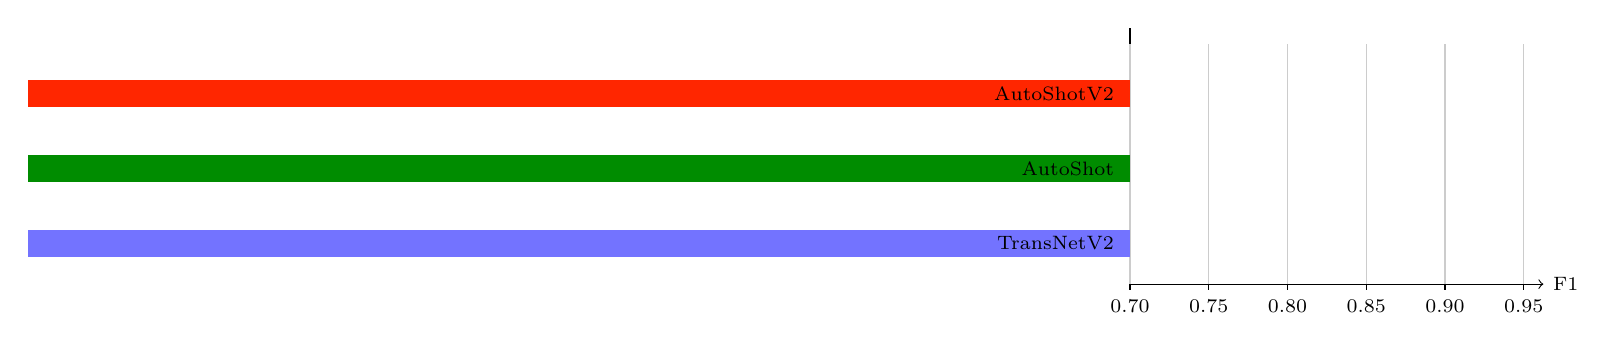
\begin{tikzpicture}[font=\scriptsize]
\def\scale{20}
\def\xzero{0.70}
\def\barh{0.34}
\pgfmathsetmacro{\valT}{20*(\PaperTransNetShotFOne-0.70)}
\pgfmathsetmacro{\valA}{20*(\PaperAutoShotShotFOne-0.70)}
\pgfmathsetmacro{\valV}{20*(\PaperASVTwoShotFOne-0.70)}
\draw[->] (0,-0.2) -- (5.25,-0.2) node[right] {F1};
\draw (0,-0.2) -- (0,3.05);
\foreach \v/\x in {0.70/0,0.75/1,0.80/2,0.85/3,0.90/4,0.95/5} {
    \draw[gray!40] (\x,-0.2) -- (\x,2.85);
    \draw (\x,-0.2) -- (\x,-0.28);
    \node[below] at (\x,-0.28) {\v};
}
\fill[blue!55] (0,0.15) rectangle (\valT,0.15+\barh);
\fill[green!55!black] (0,1.10) rectangle (\valA,1.10+\barh);
\fill[red!70!orange] (0,2.05) rectangle (\valV,2.05+\barh);
\node[anchor=east] at (-0.08,0.32) {TransNetV2};
\node[anchor=east] at (-0.08,1.27) {AutoShot};
\node[anchor=east] at (-0.08,2.22) {AutoShotV2};
\node[anchor=west] at (\valT+0.08,0.32) {\PaperTransNetShotFOne};
\node[anchor=west] at (\valA+0.08,1.27) {\PaperAutoShotShotFOne};
\node[anchor=west,font=\bfseries] at (\valV+0.08,2.22) {\PaperASVTwoShotFOne};
\end{tikzpicture}
\caption{F1-score comparison on SHOT. AutoShotV2 improves the reproduced AutoShot baseline by \PaperASVTwoVsAutoShotPP{} points and the reported TransNetV2 baseline by \PaperASVTwoVsTransNetPP{} points.}
\label{fig:shot_f1}
\end{figure}

\textbf{Controlled ablation study.} Table~\ref{tab:ablation} reports the Phase 2 ablation conducted on the cached-feature pipeline. A1 is the controlled BCE + one-hot reference. A0 is a historical AutoShot baseline evaluated with a per-dataset best-threshold sweep and should not be interpreted as a protocol-matched control. The B4 configuration is selected because it gives the strongest SHOT improvement while preserving the BBC guardrail. EMA is excluded because the available EMA experiment fine-tunes the full model on a different training pipeline.

\begin{table*}[!t]
\caption{Controlled Phase 2 Ablation (Separate from the Deploy Checkpoint)}
\label{tab:ablation}
\centering
\small
\renewcommand{\arraystretch}{1.15}
\begin{tabular}{L{3.0in}C{1.0in}C{1.0in}C{1.0in}}
\toprule
\textbf{Configuration} & \textbf{SHOT} & \textbf{BBC} & \textbf{ClipShots} \\
\midrule
\PaperControlledAblationRows
\bottomrule
\end{tabular}
\end{table*}

\subsection{Performance on Downstream Datasets}

\textbf{Effect on short-video data.} The robust improvements on SHOT indicate that AutoShotV2 effectively models short-video characteristics. The Focal Loss tackles the extreme class imbalance between boundary and non-boundary frames, while the many-hot auxiliary target supplies denser gradients around ambiguous transitions without diluting precision. Simultaneously, Gaussian smoothing heavily suppresses isolated false peaks, which frequently occur in short videos due to rapid camera motion and strong visual editing effects.

\textbf{Cross-domain behavior and ClipShots error analysis.} While AutoShotV2 transfers well to the structured documentary footage of BBC, the fixed deployment configuration reaches only \PaperASVTwoClipDeployFOne{} on the wild, open-world ClipShots dataset (Table~\ref{tab:main_results}). To diagnose this, Table~\ref{tab:clipshots_breakdown} splits ClipShots performance by transition type using the same fixed threshold $\theta=\PaperDeployThreshold$.

\begin{table}[!t]
\caption{ClipShots Breakdown by Transition Type at the Fixed Deploy Threshold}
\label{tab:clipshots_breakdown}
\centering
\small
\renewcommand{\arraystretch}{1.12}
\resizebox{\columnwidth}{!}{%
\begin{tabular}{L{1.25in}C{0.65in}C{0.65in}C{0.65in}}
\toprule
\textbf{Transition} & \textbf{Prec.} & \textbf{Rec.} & \textbf{F1} \\
\midrule
\PaperClipBreakdownRows
\bottomrule
\end{tabular}
}
\end{table}

The breakdown reveals that the primary source of degradation is the extremely low recall (4.42\%) on gradual transitions. We attribute this to three potential causes: (1) the $\pm1$ many-hot window may be too narrow for ClipShots' extended gradual transitions; (2) the temperature learned on SHOT miscalibrates the logit distribution for ClipShots; and (3) the chosen Focal Loss parameters heavily emphasize SHOT's specific hard examples over open-world editing styles.
